\chapter{Method}
\label{chap:method}

% This is the introduction to the thesis.\footnote{And this is a
% footnote.}  The conclusion is in Chapter on page
\section{Out-of-Vocabulary Model}
    \subsection{Sequence Feature Extraction}
        OOV problem is handled from quasi-generative perspective as
        aforementioned in chapter \ref{chap:intro} by using neural
        language model under assumption that there is a form that
        could generate embedding for the original embedding. Hence
        that, the original embedding is used for training the model to
        generate the embedding. In chapter \ref{chap:intro}, reasons
        why lstm could perform worse is because the hidden states is
        controlled by cell gates making the information that is
        carried on is the most recent after the cell gates decided to
        forget inputs at certain time $t$. 

        \begin{align}
            \label{eq:lstm:f_t}
            f_t &= \sigma(W_f \cdot [h_{t-1}, x_t] + b_f) \\
            \label{eq:lstm:i_t}    
            i_t &= \sigma(W_i \cdot [h_{t-1}, x_t] + b_i) \\
            \label{eq:lstm:Cc_t}
            \tilde{C}_t &= tanh(W_C \cdot [h_{t-1}, x_t] + b_C) \\
            \label{eq:lstm:C_t}
            C_t &= f_t \times C_{t-1} + i_t \times \tilde{C}_t \\
            \label{eq:lstm:o_t}
            o_t &= \sigma(W_o \cdot [h_{t-1}, x_t] + b_o) \\
            \label{eq:lstm:h_t}
            h_t &= o_t \times tanh(C_t)
        \end{align}

        Formally, when $C_t = 0$ from equation \ref{eq:lstm:C_t},
        hidden state from equation \ref{eq:lstm:h_t} will be reset to
        $0$ rendering hidden states prior to time $t$ gone. This
        problem can be solved by using bi-lstm, since bi-lstm process
        sequence in forward and reverse order making both early and
        later sequence held by the last hidden state for each forward
        lstm and reverse lstm respectively. Another problem might
        arise when we need to divide sequence into more than three
        subsequence as shown on figure \ref{fig:subsequence}. Hence
        another approach is needed since intermediate subsequence
        might get deleted or carried along with the later sequence
        even with bi-lstm.

        \begin{figure}
            \begin{align*}
                &un \vert recogniz \vert able \\
                &inter \vert national \vert ities \\
                &oto \vert rhino \vert laryngolog \vert ical \\
                &hepatico \vert chol \vert angio \vert gastro \vert stomy
            \end{align*}
            \caption{Word examples with three or more subsequences}
            \label{fig:subsequence}
        \end{figure}

        We can find many examples especially from more technical areas
        as shown on figure \ref{fig:subsequence}. Since on
        \textsc{Mimick} \cite{mimicking2017Pinter} implementation only
        the last hidden state is used for inferencing word embedding,
        another approach is proposed.

        \begin{figure}
            \begin{align*}
                unrecognizable : &unre \vert nrec \vert reco \vert ecog \vert cogn \vert ogni \vert gniz \vert niza \vert izab \vert zabl \vert able\\
                internationalities : &inte \vert nter \vert tern \vert erna \vert rnat \vert nati \vert atio \vert tion \vert iona \vert onal \vert \\
                &nali \vert alit \vert liti \vert itie \vert ties\\
                otorhinolaryngological : &otor \vert torh \vert orhi \vert rhin \vert hino \vert inol \vert nola \vert olar \vert lary \vert \\
                &aryn \vert ryng \vert yngo \vert ngol \vert golo \vert olog \vert logi \vert ogic \vert gica \vert ical\\
                hepaticocholangiogastrostomy : &hepa \vert epat \vert pati \vert atic \vert tico \vert icoc \vert coch \vert ocho \vert chol \vert hola \vert olan \vert\\
                &lang \vert angi \vert ngio \vert giog \vert ioga \vert ogas \vert gast \vert astr \vert stro \vert\\
                &tros \vert rost \vert osto \vert stom \vert tomy
            \end{align*}
            \caption{4-grams examples}
            \label{fig:4grams}
        \end{figure}

        For all subsequence to be processed, we need a method that
        accounts for all sequence yet still able to divides the whole
        sequence into subsequences. Consequently, n-grams is chosen
        because this method splits word into sequence of characters
        depends on the chosen window size as shown on figure
        \ref{fig:4grams}. Those sequences of characters then feed into
        learning algortihm. This idea is similar to how human tries to
        recognize an unseen word by reading subword that is
        understandable beforhand when no explanation or context were
        given. 

        This model then will be used to estimate OOV embeddings. In
        other words, given sets of vocabulary $\mathcal{V}$ with size
        $\vert\mathcal{V}\vert$ and pretrained embeddings
        $\mathcal{W}^{\vert\mathcal{V}\vert \times d}$ for each word
        $w_{i} \in \mathcal{V}$ that is represented as a vector $e_i$
        with $d$ dimension, the model is trained to map function
        $f:\mathcal{V} \rightarrow \mathbb{R}^d$ that minimizes $\vert
        f(w_i) - e_i
        \vert^{2}$. This approach is similar to \textsc{Mimick}
        \cite{mimicking2017Pinter} approach. The text input is
        represented as a sequence of character $[c_1, c_2, \dots,
        c_m]$ for $c_i \in \mathcal{C}$. Those sequence then
        transformed as sequence of vectors $g_i$ with $b$ dimension by
        using character embeddings $\mathcal{G}^{\vert \mathcal{C}
        \vert \times b}$. For simplicity, sequence of $[g_1, g_2,
        \dots, g_m]$ will be called $[\hat{g}]$. $[\hat{g}]$ becomes
        2-dimensional matrix that has size of $m \times b$. In
        summary, given word $w$ will be transformed using function $h$
        into $[\hat{g}]$ as shown on equation \ref{eq:word2charemb}.

        \begin{equation}
            \label{eq:word2charemb}
            h: w \rightarrow [\hat{g}]
        \end{equation}

        To process $[\hat{g}]$ like an n-grams, CNN is used. CNN is
        basically a method to do convolution on matrix by using a
        kernel $k_i^{n \times b} \in K$. This operation is represented
        with $*$ symbol. To mimick n-grams, kernel with size of $n
        \times b$ is used, producing another vector $\hat{l}$ that
        represents the value of each grams, then non-linearity is
        applied to this vector by using ReLU activation function as
        shown in equation \ref{eq:relu}.

        \begin{equation}
            \label{eq:relu}
            f(x) = ReLU(x) = max(0,x)
        \end{equation}

        Several kernel is used to learn several features for producing
        embeddings. Each of these kernel will be responsible to find
        grams that are affecting the results, thus the vector
        $\hat{l_i}$ that are results of convolution $[\hat{g}] * k_i$
        will be maxpooled to produce one number. In details, from
        given sequence of character embedding $[\hat{g}]$, only gram
        that produces the highest value when convoluted by using
        kernel $k_i$ will be processed. Since, there are $\vert K
        \vert$ number of filter, $\vert K \vert$ number of grams will
        be considered to be important to the results. Furhtermore, by
        using several window sizes for n-grams (bigram, trigram,
        etc.), more features will be able to be learned.

    \subsection{Embedding Generation}
        After the features are able to be extracted, those features
        then concatenated and fed into fully connected layer with
        output size matching the pretrained embedding $\mathcal{W}$
        dimension $d$ with non-linear activation function matching the
        maximum and minimum bound of the pretrained embedding
        $\mathcal{W}$ resulting a new embedding vector $\tilde{e}$.

        The complete process from input word, feature extraction,
        until predicting embedding is shown on figure \ref{fig:model}.
        
        \begin{figure}
            \centering
            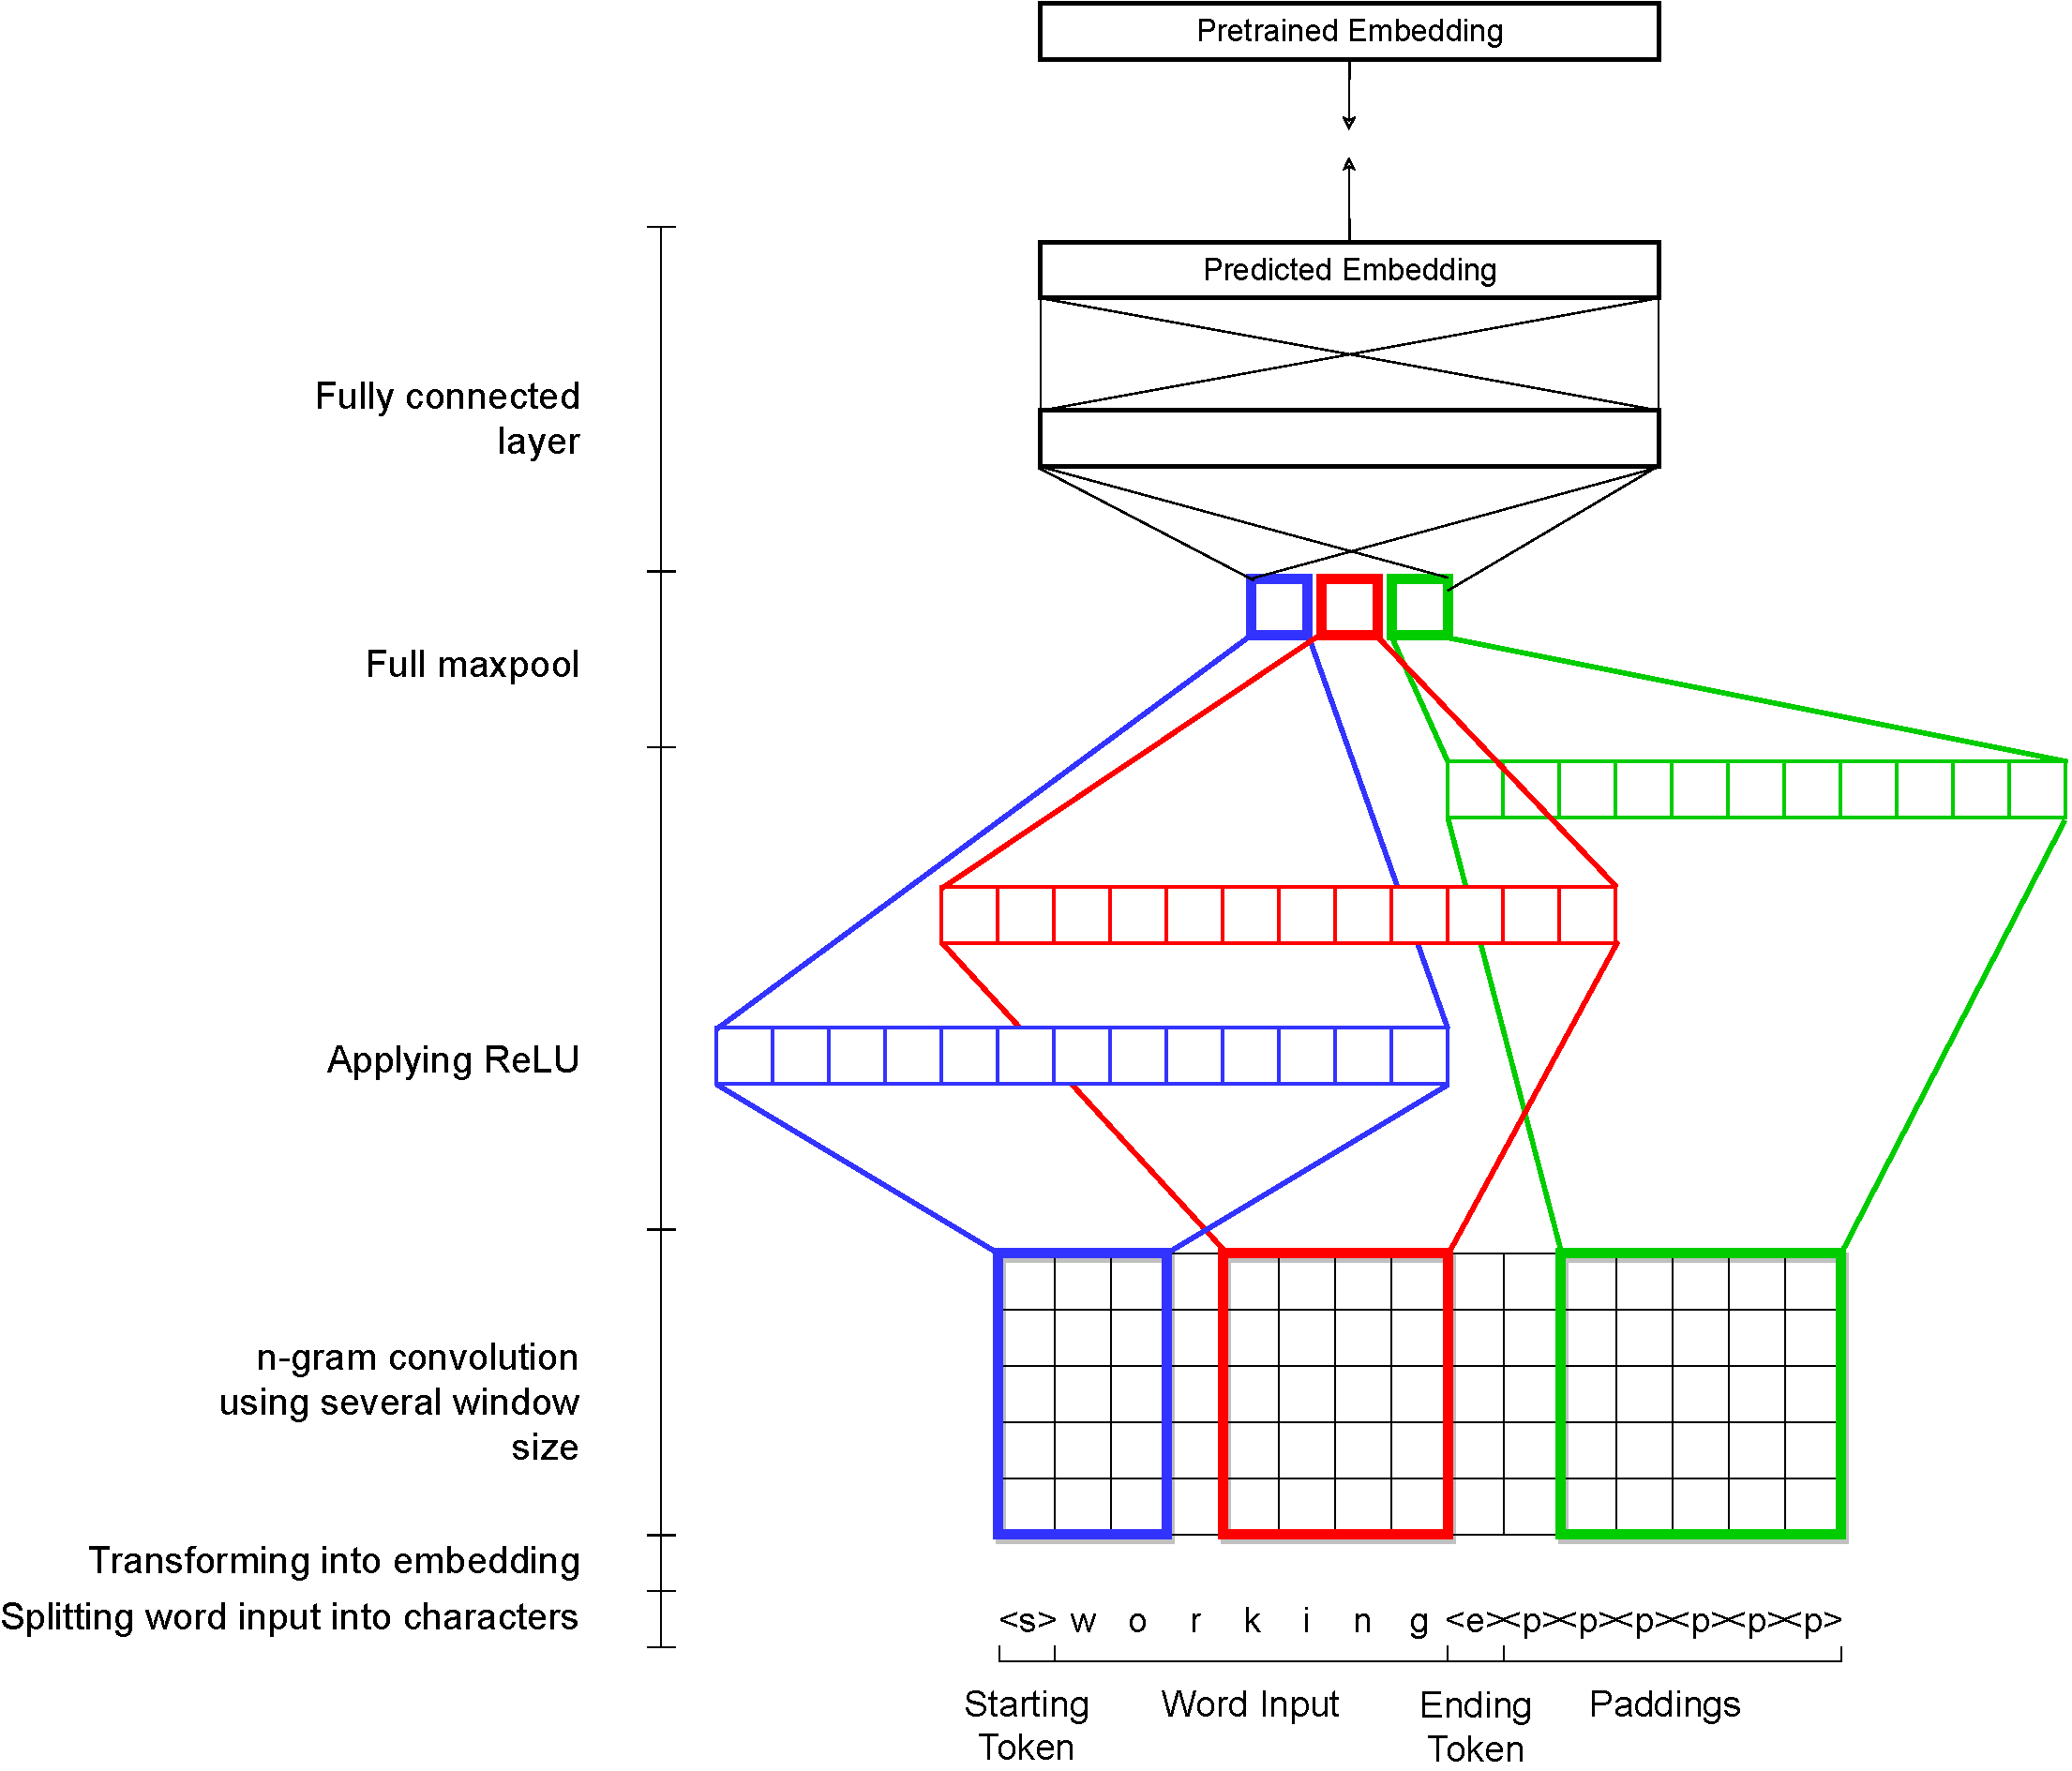
\includegraphics[width=.8\linewidth]{images/model.pdf}
            \caption{OOV Inferencing Model}
            \label{fig:model}
        \end{figure}

        On figure \ref{fig:model}, starting and ending token is added
        at the beginning and the end of the word respectfuly.
        Furthermore, padding token is added if the input word is
        shorter than the length of the input size of the model. The
        padding token is a zero vector $\vec{0}$ and $\vec{0} * k =
        \vec{0}$ for any $k$. This is to ensure that part of input
        that got padded does not goes through maxpool layer since only
        grams that has highest value can goes through the next layer
        and minimum value of ReLU is 0.

    \subsection{Error and Backpropagation}
        The output of the neural network $\tilde{e}$ then compared
        with the original embedding $e$ to learn new parameters for
        the neural network using mean squard error function as shown
        on \ref{eq:errorf}

        \begin{equation}
            \label{eq:errorf}
            Error = \frac{1}{2} \Vert e - \tilde{e} \Vert ^{2}
        \end{equation}

        The error then backpropagated to fine-tune the neural network
        parameters.
        
\section{Measuring Performance on Donwstream Tasks}
    In natural language modeling (NLP), there are several tasks that
    make used of word embedding. Hence that, the generated embeddings
    from the model can be evaluated by using those downstream tasks.
    The results then compared with the state-of-the-art OOV handling
    model \textsc{Mimick} \cite{mimicking2017Pinter}.
    
    \subsection{Part-of-Speech Tagging}
        Part-of-speech tagging or POStagging is a task of classifying
        words in sentence or corpus based on the grammatical usage of
        the word \{cite\}, for example: verb, noun, adverb, etc. Given
        sentence $S = \{w \in \mathcal{V} \vert ((w_1, t_1), (w_2,
        t_2), \dots, (w_n, t_n)\}$ with its POS-tag $t_i$, each word
        $w_i \in S$ is converted into sequence of character then each
        character is converted into character embedding $[\hat{g}]_i$
        using model represented in equation \ref{eq:word2charemb}.

        The sequence of character embeddings $[\hat{g}]_i$ then fed
        into bi-lstm with logsoftmax activation function at the output
        to get the POS-tag. To ease up computation time, adaptive
        logsoftmax is used \cite{grave2018efficientsoftmax}. Instead
        of calculating the whole classification, the frequent and
        infrequent classes are separated thus there are many chance
        that only frequent classes needs to be calculated. The
        complete process of postagging process is shown in figure
        \ref{fig:postag}.

        \begin{figure}
            \centering
            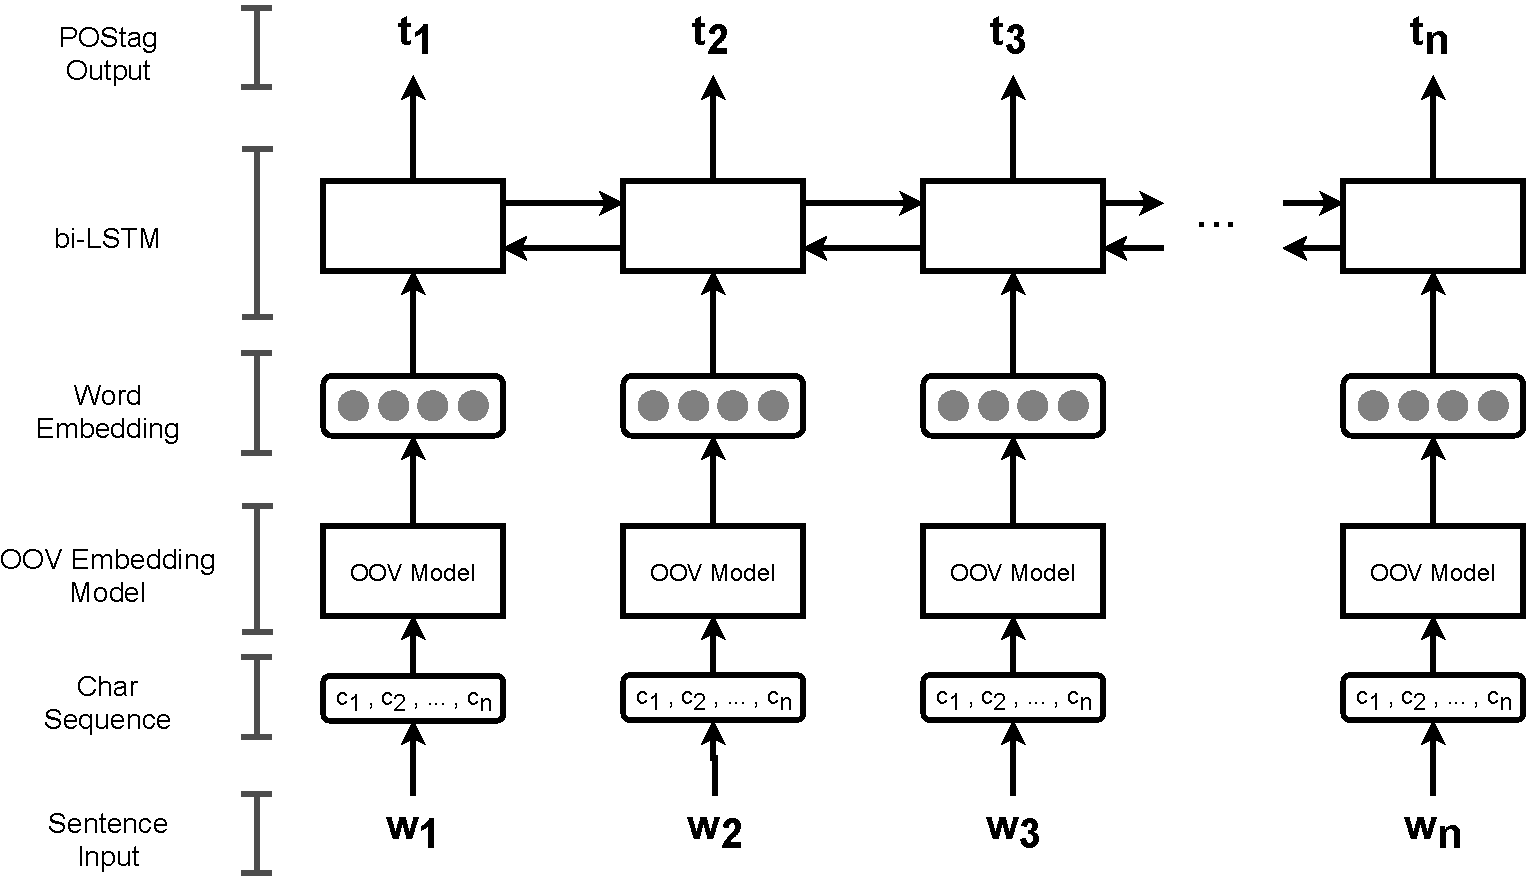
\includegraphics[width=.8\linewidth]{images/postag.pdf}
            \caption{Postagging Process}
            \label{fig:postag}
        \end{figure}
 
    \subsection{Word Similarity Tasks}
        Word similarity tasks is basically task to evaluate the
        similarities between two words based on human given scores.
        Generally, several human subject were given pairs of words and
        asked to score its similarities. Those scores then will be
        used to determine the agreements between subjects that certain
        word pairs have stronger connection and the others are weaker.
        In order to calculate the agreements between the OOV generated
        embedding and the data that is scored by human, Spearman's
        rank correlation coefficient is used. Firstly, given a pair
        $(w_1, w_2)$, the cosine distance of the embedding based on
        the generated OOV model between $e_1$ and $e_2$ for $w_1$ and
        $w_2$ respectfuly, are calculated using equation
        \ref{eq:cosinesim}. 

        \begin{equation}
            \label{eq:cosinesim}
            cosine\ similarity = \frac{e_1 \cdot e_2}{\Vert e_1 \Vert \Vert e_2 \Vert}
        \end{equation}

        After all of the cosine distance for all pairs are calculated,
        Spearman rank's correlation from the dataset and the generated
        embedding are calculated by using equation \ref{eq:spearman}
        and by using equation \ref{eq:spearmantied} when no tied ranks
        exists.
        
        \begin{align}
            \label{eq:spearman}
            \rho    &= \ddfrac{n\sum_{i=1}^n u_i v_i - \Bigg( \sum_{i=1}^n u_i \Bigg) \Bigg( \sum_{i=1}^n v_i \Bigg)}{\sqrt{\Bigg[ n \sum_{i=1}^n u_i^2 - \Bigg( \sum_{i=1}^n u_i \Bigg)^2 \Bigg] \Bigg[ n \sum_{i=1}^n v_i^2 - \Bigg( \sum_{i=1}^n v_i \Bigg)^2 \Bigg] }}\\
            \label{eq:spearmantied}            
                    &= 1 - \ddfrac{6 \sum_{i=1}^n d_i^2}{n(n^2 - 1)}\ \text{where}\ d_i = u_i - v_i
        \end{align}
